\documentclass[12pt]{article}
\usepackage {amsmath}
\usepackage {amssymb}
\usepackage {epsfig}
\usepackage {bm}
\usepackage {indentfirst} %indent the first par after section
\usepackage{setspace} 
\usepackage{color}
\usepackage{multirow}
\usepackage{cite}
\usepackage{eurosym}
\usepackage{graphicx}
\usepackage{soul}

\usepackage{array}
\newcolumntype{L}[1]{>{\raggedright\let\newline\\\arraybackslash\hspace{0pt}}m{#1}}

%\doublespacing
\oddsidemargin0cm
\topmargin-2cm     %I recommend adding these three lines to increase the 
\textwidth16.5cm   %amount of usable space on the page (and save trees)
\textheight23.5cm

\RequirePackage{lineno}
%\setlength{\linenumbersep}{6pt}
\linenumbers

\def\sNN{\sqrt{s_{\rm NN}}}

\def\la{\left< }
\def\ra{\right> }
\def\mean#1{\ensuremath{\la#1\ra}}
\def\meanabs#1{\ensuremath{\la|#1|\ra}}
\def\meankv#1{\ensuremath{\la#1^2\ra}}
\def\rms#1{\meankv{#1}}
\def\sqrtrms#1{\ensuremath{\sqrt{\meankv{#1}}}}
\newcommand{\snn} {\ensuremath{\sqrt{s_{\rm NN}}}}
\def\ptq#1{\ensuremath{\hat{p}_{\rm T#1}}} 
\def\ptqkv#1{\ensuremath{\hat{p}^2_{\rm T#1}}} 
\def\vptq#1{\ensuremath{\vec{\hat{p}}_{\rm T#1}}} 
\newcommand{\s} {\ensuremath{\sqrt{s}}}
\def\tev{\mbox{~TeV}}
\def\gev{\mbox{~GeV}}
\def\gevc{\mbox{~GeV/$c$}}
\def\eg{{\it e.g.}}
\def\etc{{\it etc}}

\def\pt#1{\ensuremath{p_{\rm T#1}}} 
\def\ptkv#1{\ensuremath{p^2_{\rm T#1}}} 
\def\vpt#1{\ensuremath{\vec{p}_{\rm T#1}}} 

\def\kt#1{\ensuremath{k_{\rm T#1}}} 
\def\ktkv#1{\ensuremath{k^2_{\rm T#1}}} 
\def\vkt#1{\ensuremath{\vec{k}_{\rm T#1}}} 

\def\jt#1{\ensuremath{j_{\rm T#1}}} 
\def\jtkv#1{\ensuremath{j^2_{\rm T#1}}} 
\def\vjt#1{\ensuremath{\vec{j}_{\rm T#1}}} 

\newcommand{\mz} {\mean{z}}
\newcommand{\zt} {\ensuremath{z_{\rm t}}}
\newcommand{\mzt} {\mean{\zt}}
\newcommand{\za} {\ensuremath{z_{\rm a}}}
\newcommand{\mza} {\mean{\za}}
\newcommand{\xe} {\ensuremath{x_{\rm E}}}
\newcommand{\xh} {\ensuremath{x_{\rm h}}}
\newcommand{\xhq} {\ensuremath{\hat{x}_{\rm h}}}
\newcommand{\zkt} {\ensuremath{ \mean{\zt}\sqrtrms{\kt{}} }}
\newcommand{\xzkt} {\ensuremath{ \xhq^{-1}\mean{\zt}\sqrtrms{\kt{}} }}
\newcommand{\xzktfull} {\ensuremath{ \xhq^{-1}(\kt{},\xh)\mean{\zt(\kt{},\xh)}\sqrtrms{\kt{}} }}
\newcommand{\pp} {pp}
\newcommand{\ppb} {p--Pb}
\newcommand{\pbpb} {Pb--Pb}
\newcommand{\auau} {Au--Au}

\def\defn#1{{\color{red} #1}}
\def\tred#1{{\color{red} #1}}
\def\tblue#1{{\color{blue} #1}}

\hyphenation{ALICE}

%\title{Research Plan}
\title{Probing Soft-Hard Interactions in Relativistic Heavy Ion Collisions with ALICE Experiment at CERN LHC}
\author{PI : Jan Rak}

\begin{document}

\maketitle
\begin{flushleft}
%Principal investigator : Jan Rak \\
Duration of the project: 48 months, 1.9.2018 -- 31.08.2022\\
Site of the research: Department of Physics, Jyv\"askyl\"a University and CERN
\end{flushleft}

%\centerline{Version 0.1}

%\tableofcontents

%!TEX root = ResearchPlan_v2.tex

\section{Rationale}%%%%%%%%%%%%%%%%%%%%%%%%%%%%%%%%%%%%%%%%%%%%%%%
\label{sec:rationale}
The main emphasis of the ultra-relativistic heavy ion collisions (URHIC) is to study deconfined phase of the strongly interacting matter, the Quark-Gluon Plasma (QGP). Current widely accepted view is that the existence of the phase transition to QGP was experimentally established based on the analysis of  Au--Au collision data at center-of-mass energy $\sNN=200$~GeV measured at Relativistic Heavy Ion Collider (RHIC) located in Brookhaven Nation Laboratory, USA.

At the beginning of 2010, the Large Hadron Collider (LHC) at CERN became fully operational and the first Pb--Pb collisions at $\sNN=2.76$~TeV were recorded.  These measurements strenghtened the observations already made at RHIC, but the most importantly, they opened many new avenues to more detailed observations. 
The extreme center of mass energies accompanied by large luminosity delivered by the LHC machine allow heavy ion physics to enter an era of precision measurements. 
The proof of QGP existence, down to a level where there is hardly any doubt left, was the first step. 
Now we have started to map out more detailed features of this phase transition.
%, like the transport coefficients of the matter created in URHIC. 
This application will present an ambitious plan to pin down temperature dependence of the shear viscosity to entropy ratio $(\eta/s)$ and to search for a signatures of Mach cone shock waves, that have a long time anticipated to be found but have proven out to be difficult to observe. 
Observation of the Mach cone waves could uncover a direct experimental access to the speed of sound in QGP, one of the most fundamental property characterizing the deconfined state of matter. 
These objectives and measurement techniques will be discussed in Section~\ref{sec:objectives}.

The temperature dependence of the $\eta/s$ has some generic features that most of the known fluids obey. One such general behavior is that the ratio typically reaches its minimum value close to the phase transition region \cite{PhysRevLett.98.092301}. One can argue, using kinetic theory and uncertainty relations~\cite{PhysRevD.31.53}, that $\eta/s\sim0.1$ would be an order of magnitude for the lowest possible shear viscosity to entropy ratio in nature. Later it was found that one can calculate an exact lower bound $(\eta/s)_{\rm min}=1/4\pi\approx0.08$ using the AdS/CFT correspondence~\cite{PhysRevLett.94.111601} to certain class of conformal field theories. Hydrodynamical simulations supports as well the view that hot QGP matter indeed is close to that limit~\cite{Gale:2012rq}. This in turn may have an important implications to other fundamental physics goals. It is argued that such a low value might imply that thermodynamic trajectories for the expanding matter would lie close to the QCD critical end point, which is another subject of intensive experimental quest~\cite{PhysRevLett.98.092301}.
%which in turn would gain better prospects to search of critical end point~\cite{PhysRevLett.98.092301}.

Our group is fulfilling a strong involvement that Finland has in the ALICE experiment at CERN LHC. On top of that, two members of our group, the PI and senior researcher DongJo Kim, are members of the PHENIX experiment at RHIC, but those activities are not explicitly advanced with this application. Finnish participation to ALICE started with hardware oriented tasks. Helsinki Institute of Physics (HIP) was involved with bonding and assembly of the Silicon Strip Detector (SSD) and this project was successfully completed in 2006. Department of Physics at University of Jyv\"askyl\"a (JYFL) took the main responsibility in designing, building and maintaining the T0 fast timing detector that has provided not only a precise timing of the interaction but served also as a vertex, trigger and luminosity detector. The very successful T0 project is still on-going until the end of current LHC Run2 that finishes in December 2018. After that, ALICE will go trough a major upgrade where all central detectors are upgraded and also forward detectors T0, V0 and FMD will be merged into a new Fast Interaction Trigger detector  (FIT). The project leader of the T0 detector, Wladyslaw Trzaska, is also the project leader of the FIT. 
This detector system should be finished and commissioned during the Long Shutdown 2 (LS2) that takes place in 2019-2020. The Finnish participation to this effort is promoted by another Academy project application by Wladyslaw Trzaska in this same call.

Our group has designed and built the Trigger Region Units (TRU) system which derives the fast level-0 trigger from the electromagnetic calorimeter (EMCal) data. It provides the L0 single photon trigger to ALICE Central Trigger Processor (CTP) and it is combined into level-1 single photon and jet trigger. 
%In the case of single photon L1-trigger, STU does a logical OR action over all the TRU units. EMCal has also a jet trigger with higher patch size and trigger threshold. 
These triggers are very essential to all rare trigger data taking in the ALICE experiment. This project was so successful that the main TRU trigger design was adapted into another calorimeter, PHOton Spectrometer (PHOS), and also to Di-jet CALorimeter (DCAL) that is an extension of EMCal located in opposite side in azimuth. Both maintaining the L0 trigger and promoting analysis with EMCal+DCAL calorimeter systems are key ingredients of this application.
%, both extremely important Finnish contributions to the ALICE experiment. 

Our group and particularly the HIP detector laboratory are also involved with the upgrade of the ALICE Time Projection Chamber (TPC). The TPC is the main tracking detector of the central barrel ($|\eta|<0.9$) and is optimized to provide charged particle momentum measurements down to 50~MeV/$c$ with excellent two-track separation, particle identification trough $dE/dx$ and vertex determination. The current design of the TPC allows the heavy ion data taking with maximum rate of 500 Hz. The rate is mainly limited by TPC gating grid that is needed to prevent the ion back flow to the drift volume. 
However, after LS2, the luminosity in heavy ion collisions will require the readout rate to be boosted up to 50 kHz. 
The goal of the TPC upgrade is to replace the multi-wire proportional readout chambers with the Gas Electron Multiplier (GEM) technology that allows the increase of the readout rate and to preserve PID capabilities and excellent momentum resolution.

Our group is responsible for the Quality Assurance of the whole 150 m2 of GEM foils. The QA work is done at the detector laboratory in HIP. Recently the same setup, developed by our team in HIP, has been copied into Wigner Institute in Budapest. The GEM foil studies will finish around June 2018, well before LS2 starts in December. \textcolor{blue}{OUR RESPONCIBILITIES IN FUTURE?}

To fulfil our responsibilities in hard ware duties, both the post doc and PhD-student will use fraction of their worktime in the hard ware tasks, although the physics analysis will be the main duty for them both. The post doc will participate into TPC upgrade during the LS2 and perform the trigger commissioning when the Run 3 starts. The hired PhD-student (Jasper Parkkila) will also deliver is service task to ALICE experiment in TPC upgrade tasks. Timetables will be elaborated in the later parts of this application.


\section{Objectives and expected results} %%%%%%%%%%%%%%%%%%%%%%%%%%%%%%%%%%%%%%%%%%%%%%%
\label{sec:objectives}

\subsection{Objectives of the research}

The large elliptic flow discovered at RHIC energies continuous to increase also in the highest beam energy $\sNN=5.02$~TeV currently reached in LHC. This has been predicted by calculations utilizing viscous hydrodynamics~\cite{PhysRevLett.99.172301} and microscopic transport models ~\cite{PhysRevLett.101.082302}.  These calculations also demonstrated that the shear viscosity to the entropy density ratio ($\eta/s$) of strongly interacting matter is close to a universal lower bound $1/4\pi$~\cite{PhysRevLett.94.111601} in heavy ion collisions at RHIC and LHC energies. One of the open questions is weather the viscosity of the matter is small enough that a high momentum parton, that would be supersonic in the QGP, could trigger a Mach Cone shock wave to the matter. Large viscosity might damp the shock wave before the freezeout of the fireball and hence it may not show up in the final (hadronic) observables~\cite{Bouras:2010nt,Bouras:2012mh,PhysRevC.90.024904}.

Early studies expected that the Mach cone shock wave would be observed as a double-hump structure in the away-side of azimuthal correlations~\cite{jabref}, relating to a opening angle of the cone. However, it turned out that the observed structure was explained fully by odd Fourier components of hydrodynamical flow that arises from initial geometry fluctuations 
in the collision of the relatively large nuclei~\cite{Luzum:2012wu,ALICE:2011ab}. This breakthrough started a rapid development in flow observables and analysis that has started a series of precision flow measurements. The simultaneous description of higher-order flow harmonics ($v_{n}$) and their \pt{}\ dependence turned out to provide important constraints to both the $\eta/s$ and to initial fluctuations~\cite{Luzum:2012wu}. Even further, correlations between magnitudes of two different flow harmonics, that already are very subtle flow measurements, can provide sensitivity to the temperature dependence of $\eta/s$ in the state-of-the-art hydrodynamic calculations~\cite{Niemi:2015qia} in combination with individual flow coefficients~\cite{ALICE:2016kpq}. The higher order ($v_5$ and higher) to lower order ($v_2$ or $v_3$) harmonic correlations can help to understand the viscous correction to the momentum distribution at freeze-out, which is one of the largest current uncertainties in the hydrodynamic models~\cite{PhysRevC.86.044908,Niemi:2015qia}. All in all, the advanced flow measurements are timely and very intensive line of research, and have significant potential to increase our understanding of QCD matter.

The full jet reconstruction in heavy ion environment has also gone trough rapid progress over the LHC time, see e.g. \cite{Abelev:2013kqa}. This has brought hydrodynamic response to the jet quenching again into the spot light because it affects various observables in detailed measurements with full jet reconstruction. The enhancement of low transverse momentum particles away from the quenched jets can be interpreted as a consequence of the energy-momentum transport by the Mach cone~\cite{Tachibana:2014lja}. 
The soft particles from the medium excitation affect also the fragmentation functions and the jet transverse profile~\cite{He:2015pra}.

Significant effort has been made to understand the measured fragmentation functions and the jet structure in heavy ion collisions~\cite{Chatrchyan:2011sx,Chatrchyan:2013kwa,Chatrchyan:2014ava,Adam:2015ewa,Khachatryan:2016erx}. Although the theory of parton energy loss has been successful in describing single particle spectra, namely the nuclear modification factor $R_{AA}$~\cite{Aamodt:2010jd}, the theoretical understanding of the in-medium parton shower is not yet fully achieved ~\cite{PhysRevLett.106.122002}. Therefore, in the absence of a consistent theory of jets in a medium, phenomenological studies of jet observables have relied to a large extend on modeling of medium modified parton showers~\cite{Armesto:2008qh,Renk:2010zx}. One can say that detailed modeling of medium modified jets, with a realistic hydrodynamical medium description such that the jet is coupled to the expanding medium, does not yet exists.

It has been realized that already the distribution of interaction vertices, where the hard parton was produced, can blur out the double-hump structure in two-particle correlations and hence make a straightforward observation of Mach cone more difficult~\cite{Tachibana:2015qxa}. Hence one needs to find out and exercise more detailed observables to pin down so called hard-soft interactions between the hard parton (that initiates the jet in the final state) traversing the medium of soft particles. The ambitious goal of this application is to make significant experimental progress towards this goal. Soft-hard interactions in general are dependent of the key features of the QGP, such as fluidity, sound velocity, viscosity and stopping power.

The practical implementation will be based on refining further the current flow measurements. Like discussed above, event-by-event correlations between magnitudes of different flow harmonics have turned out to be rich source of information and constraints to QGP properties. We aim to bias the event selection in such away that the event contains a single hard jet or a di-jet. This would be a new direction compared to presently studied event shape engineering, where one selects high-$v_2$  events for more detailed hadron correlation studies~\cite{ALICE:2016kpq}. Investigating modifications of various flow harmonic measurements in the presence of hard (di-)jet, as compared to just centrality selected collisions, requires a high statistics data sample and definitely makes use of the EMCal triggered data samples in \pbpb\ collisions.

This applications involves a post doc and PhD-student. Both would have hardware duties, but the main emphasis would be on the analysis goals. The flow correlations would be the PhD students thesis topic. Post doc would concentrate first on the jet studies and then later would lead the research in combining the jet and flow studies. Obvious risk is that at the end we cannot find strong signals that could be clearly related to hard-soft interactions. However, the plan is designed such that well defined and meaningful milestones can be set up. These will be refined in later parts of this application.

\subsection{Effects and impact beyond academia}

This application belongs into basic research that does not aim to immediate applications outside academia. However, CERN research has been very beneficial for example through its technology program, which directly benefited (Finnish) companies particularly during the LHC construction phase. CERN projects act as a driving force of technological advancement that may find their way for example to medical instrumentation. One observes in practice aging of electronics in high radiation environment.

The experimental techniques and various tools used for the data analysis are of common interest for rapidly developing industry since they require modern technologies. For example, a field-programmable gate array (FPGA) coding is our main part of the trigger logic development for EMCal trigger. Specific applications of FPGAs include digital signal processing, software-defined radio, ASIC prototyping, medical imaging, computer vision, speech recognition, cryptography, bioinformatics, computer hardware emulation, radio astronomy, metal detection and a growing range of other areas.

Technological aspects related to data acquisition (DAQ) systems for particle physics experiments following the natural path of the signals from the detector to the data processing are also broad interest of modern high-tech companies and any researches in general. The computer programming languages and software tools we are using in everyday for our researches are also needed skills for professionals in companies  who deal with the database, IT and many others. One concrete example would be mining of huge amounts of data in GRID environment. Two former members of our group have been hired to private sector based on their experience with the big data and programming skills.

\subsection{Publication plan}

ALICE Collaboration has made an effort to make the publication process such that all preliminary results that the collaboration produces would be effectively published. In general, CERN experiments publish in high impact journals and the internal review process helps to polish the results to very high quality. CERN has committed that all results will be published also in open access, which concretely promoted through SCOAP$^3$ project\footnote{SCOAP$^3$ stands for Supporting Consortium for Open Access Publishing in Particle Physics, see https://scoap3.org}. In practice, the scientific papers go to arXiv at the same time they are submitted into journal. Public analysis note and technical reports are published openly in the CERN's own CDS-database.

\section{Research methods and material, support from research environment} %%%%%%%%%%%%%%%%%%%%%%%%%%%%%%%%%%%%%%%%%%
%%%%%
\label{sec:researchmethods}

The field of heavy ion physics has very vivid cross talk between theoreticians and experimentalist world wide. This is seen, for example, in the development of the analysis methods~\cite{Poskanzer:1998yz,Bilandzic:2010jr}, detailed phenomenological modeling such that underlying theories are compared with the data~\cite{Burke:2013yra,Renk:2011gj,Niemi:2015qia} and tuning and development of the heavy ion event generators~\cite{Gyulassy:1994ew,Lin:2004en,Lokhtin2006}. For example, in the flow analysis, this interplay has been realized in the correlations between flow harmonics~\cite{Poskanzer:1998yz,ALICE:2011ab} and event plane angles~\cite{Aad:2014fla,Bhalerao:2014xra} that are crucial starting points in this application. Two particle correlations have been a long established tool in heavy ion physics~\cite{PhysRevLett.95.152301,PhysRevLett.97.052301} and this line is currently developing to various jet-hadron correlation, see e.g.~\cite{Khachatryan:2016tfj}. The research tools and methods are timely. They are under significant international interest and development, and belong to past experience of our group.

Observing the Mach cone in heavy ion collisions, or studying hard-soft interactions in general, has been a goal for a long time. After the observed cone-line structure in azimuthal correlations turned out be explained by the collective flow~\cite{ALICE:2011ab} and more detailed study of distribution of the hard interaction vertices was found out to smear the signal~\cite{Tachibana:2015qxa}, it is clear this proposal possesses a risk the positive observation may not come. However, the development in the field is astonishing, taking for example the correlations of the flow coefficients now measure correlations strengths that are order of part per million over the average values~\cite{ALICE:2016kpq} and the phenomena have a valid theoretical description. Heavy ion physics is clearly entering to the precision measurements where large statistics measurements enable extraction of weaker signals. Also, the steps towards the goal will provide results that are very valuable in discriminating and refining the current phenomenological models.

Obviously CERN is one of the best environments in the whole world to carry out this research. In ALICE experiment, the physics analyses are performed in the Physics Working Groups (PWG) that collect world wide researchers that are interest in a particular topic. Our group is involved in PWG's for correlation and flow analysis, and a PWG for jet analysis. The analysis work is supported and steered by the PWG's and a good interaction in the group provides a constant feedback and steady path to publish the results.

Department of Physics in Jyv\"askyl\"a has a long tradition in heavy ion physics dating back to early works by Vesa Ruuskanen and his collaborations \cite{VonGersdorff:1986tqh}. The experimental involvement started heavily when Jyv\"askyl\"a and HIP committed themselves to design and build the T0 timing detector to ALICE and production SSD modules to ALICE inner tracker~\cite{Dellacasa:1999kf}. Currently particle physics, and ultra-relativistic heavy ion collisions, is one of the main research lines in Jyv\"askyl\"a to which the department is fully committed itself. In wider perspective, it is also part of the "Structure of Matter with Accelerator Methods" to which Academy of Finland has granted profiling funding to University of Jyv\"askyl\"a. In theory side we have a strong group lead by Academy project leader and professor Kari Eskola and ERC Consolidator grant holder Tuomas Lappi, both internationally recognized experts in the heavy ion physics. Our group governs the Finnish participation to ALICE experiment trough a project in Nuclear Matter program in HIP. Together with the local cosmology and neutrino physics group, the department has build an extensive teaching program in various topics in particle physics up to a high level post graduate courses both in experimental and theoretical side. We have a common seminar with the theory group and untrammeled interaction between the groups.

Research results in this project come from analyzing the data with self-written codes. In following I will provide a brief description on how the data management goes in practice. 
The raw data for this project (order of 10 petabytes of raw data every calendar year) will be collected by the ALICE experiment at CERN. 
%The LHC project at CERN will collect huge amounts of data. For example, ALICE experiment will collect order of 10 petabytes of raw data every calendar year. 
Preservation and availability of this data is under the CERN's own data management plan and taken care of internationally.

All data measured by the ALICE experiment are available in LHC grid. Team of professionals will mine the raw detector data into more user friendly analysis files (Analysis Object Data (AOD)), where one has physical objects, like charged tracks or calorimeter clusters, from all good runs and events in some data taking periods. These files are stored, backed up and made available by CERN. Every research team in the collaboration can participate into Quality Assurance of the data and AOD's are updated by the findings of the analyzers.

In practice that data analysis has following guidelines: All the analysis code is written to so called AliRoot\footnote{http://aliroot-docs.web.cern.ch/aliroot-docs/} code packet, which is a GIT-repository (version control system) governed by CERN. Every analyzer belongs into some Physics Working Group (PWG) under which she develops her own analysis code. All the analysis code is first tested locally and then committed into this experiment wide GIT-repository, assuming that it passes quality criteria set by the experiment. By the latest at this point, the code that analyzer produced is stored and backed up with full version control. 

In ALICE, the data is recommended to be mined in so called ``lego train framework'' \cite{Zimmermann:2015owa}. This means that the analysis code that is committed into AliRoot will run over the desired data sets in the LHC grid environment semi-automatically and user can collect the ready analysis results from the data mining from grid to his local computer.

In the final state, analyzer develops an analysis and Figure plotting macro locally to reach the very final analysis results. These results are first approved by the PWG and later exposed to the whole collaboration to get the ALICE preliminary status. All analysis must be accompanied with very detailed internal analysis note. This note together with all analysis and figure plotting macros are stored in the internal pages of the ALICE experiment and hence all the documentation and all the final codes are fully stored, backed up with version control and made available to the collaboration. LHC experiments prepare also public analysis notes where certain analysis details, that will not come out along papers, are made publicly available. CERN has committed itself to fully open access publishing of all the scientific results obtained at CERN.

\nopagebreak


%!TEX root = ResearchPlan_v2.tex

\section{Ethical issues}

There is no need of ethical considerations in any of the research done in ALICE experiment at the Large Hadron Collider in CERN.


\section{Implementation: schedule, budget, distribution of work} %%%%%%%%%%%%%%%%%%%%%%%%%%%%%%%
\label{sec:implementation}

Figure~\ref{fig:LHC-mid-term} shows the medium term running plan of the LHC. 
%%%%%%%%%% BEGIN FIGURE %%%%%%%%%%%%%%%%
\begin{figure}[htbp]
   \centering
   \resizebox{15cm}{!}{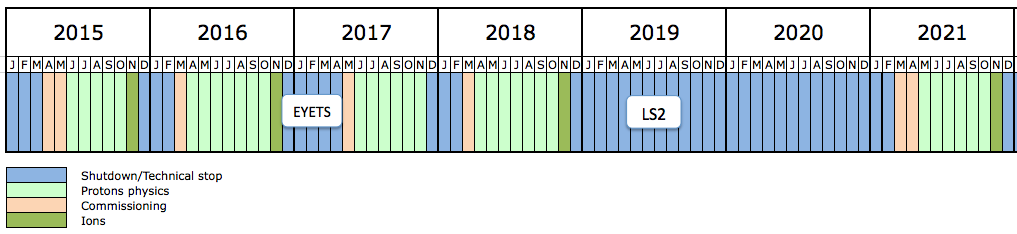
\includegraphics{LHC-medium-term.png}}
   \caption{Current draft of the medium term LHC running plan.}
   \label{fig:LHC-mid-term}
\end{figure}
%%%%%%%%%% END FIGURE %%%%%%%%%%%%%%%%%
We took lead-lead data in 2015 and will measure proton-lead at the end of 2016. After that there will be a longer end-of-the-year shutdown (EYETS). The purpose of the EYETS is to reduce workload that LHC would otherwise face during the Long Shutdown 2 (LS2) starting December 2018. Just before the LS2, there will be one more lead-lead campaign that ends the Run 2.

Year 2010 and 2011 heavy ion data (Run1) was taken at lower energy, $\sNN=2.76$~TeV, and 2015 data (Run2) with higher energy, $\sNN=5.02$~TeV. As ALICE reached the nominal design luminosity in 2015, that data set has 100 times more statistics compared to 2011 data set, that already was larger than 2010. However, we also experienced tracking problem in TPC due to accumulated space charge in high luminosity runs. It has turned out that calibration of 2015 data needs significantly more effort than earlier data sets. This may indicate that it will take substantial time in 2019 before 2018 heavy ion run results will be in hands of the analyzers. Due to these reasons, it may be that the 2015 heavy ion data will be the main source of data for analyzers that are promoted with this application. If LHC will not go to $\s{}=14$~TeV in proton-proton during Run 2, then for sure the 2018 heavy ion run will be with the same energy, $\sNN=5.02$~TeV. If all goes well, then both the 2015 and 2018 data sets are in good shape for physics analysis in beginning of 2020 and we should have significant statistics at hand.

Related to this application, currently our group is involved with completing of flow and jet analysis with Run1 and Run2 data. Two of our PhD students Jussi Viinikainen and Marton Vargyas are finishing analysis of jet fragmentation in p-Pb and Pb--Pb collisions. In September 2016, J. Viinikainen  presented his results in the parallel talk at the Hard Probes conference in Wuan, China. The first paper on correlations between magnitudes of two different flow harmonics is just accepted in Phys. Rev. Lett.~\cite{ALICE:2016kpq} and the manuscript was selected a PRL Editors' Suggestion. DongJo Kim was one of the main contributors for this paper in ALICE and he is the chair of the 2$^{\rm nd}$ paper which will contain higher order flow harmonics correlations as well as the transverse momentum and rapidity dependence of the correlations. This 2nd paper is currently being prepared for collaboration review and these results will be presented in the "Quark Matter 2017" conference in February 2017. 

%%%%%%%%%%%%%% TABLE : TimeTable for the analysis %%%%%%%%%%%
%\begin{table}[htdp]
\begin{table}[htp]
\caption{Rough timetable for expected milestones in the analysis.}
\begin{center}
\begin{tabular}{ L{1.6cm} | L{11.5cm} | L{1.0cm} }
Assigned & Task & Year \\
\hline
 & Reproducing flow observables from Run2 5TeV data &  2017 \\
PhD-     & Finishing the analysis on higher harmonic flow correlation  & 2018\\
student & Paper proposal from higher harmonic flow correlation & 2019 \\
 & Finishing paper and thesis on higher harmonic flow correlation & 2021 \\
 & PhD-studies (40 cr) and 6 months of Service Work (20 cr) &  \\
\hline
 & Charged hadron and jet $p_{T}$ spectra reconstruction & 2017 \\
 & Establishing hypothesis for various event section criteria of jets  & 2018 \\
Post doc & Systematic studies on for various event section criteria of jets & 2019 \\
 & Final paper for "Interplay of Hard and Soft Physics"  & 2021 \\
 & EMCal trigger maintenance & cont. \\
\hline
 Together& Systematic studies on flow observables for various event section criteria of jets & 2020 \\
\hline
\end{tabular}
\end{center}
\label{tab:timetable}
\end{table}
%%%%%%%%%%%%%% END TABLE %%% %%%%%%%%%%%

As the pre-requisites studies for correlations of flow harmonics from Run1 will be finalized in 2017, quite likely close to beginning of this application period, we will be in very good position to start the analysis outlined here. Table~\ref{tab:timetable} shows the outline we find realistic for studies that will combine current flow analysis to event selection bias coming from presence of hard jets.

One should note that the above is only for the analysis. Post doc will have to use fraction of his/her time for the EMCal trigger maintenance. PhD-student must give equivalent of total of 6 months of full working time to ALICE experiments service work. Regarding our obligations, the PhD student will be quite likely involved also in the TPC upgrade activities. The exact timing either to LS2 or preceding QA work will depend on the need. Our group members have to participate into our institutional share of the ALICE shift load during running of the experiment.

This applications has mainly salary and mobility allowances together with some travel costs which makes the budgeting in principle rather straightforward. We apply here a salary for a post doc and PhD-student positions, see Table~\ref{tab:money} for average yearly costs.
%%%%%%%%%%%%%% TABLE : MONEY %%%%%%%%%%%
\begin{table}[htp]
\caption{Main expenses in a yearly budget.}
\begin{center}
\begin{tabular}{l|l|r|r|r|r}
Position & Assignment & Salary & Mobility & Travel & Tot. cost\\
& & month & year & year & year \\\hline
Post doc & Analysis + EMCal running    & 3'350 & 12'600 & 2'000 & 116'762\\
PhD student & Analysis + TPC upgrade & 2'200 &  See text   & 2'000 & 69'090 \\
PI & Project leading & 6'000 &  See text   & See text & 22'870 \\
\multicolumn{5}{r}{Average full cost/year} & 208'722  \\
\end{tabular}
\end{center}
\label{tab:money}
\end{table}
%%%%%%%%%%%%%% END TABLE %%% %%%%%%%%%%%
As the post doc should be 100~\% of the time at CERN, due to planned responsibilities in EMCal running and maintenance, he/she would need (minimum) of $12\times1050$~\euro$/{\rm m}=12600$~\euro\ per year the mobility money. Also the PhD-student needs to spend significant time in CERN to perform the service work duties, do shifts and interact with Physics Working Group. Due to project size limitations, we could not embed his/her mobility costs to this application. We will use some other source, like annual HIP ALICE project resources, to this purpose.

Currently the post doc is not named, so this position would go into international call. Quite likely a suitable candidate could be a recently defended PhD inside the ALICE experiment, who has background in flow or EMCal jet analysis. He/she would then be very familiar with the experiment and analysis environment. Our group has a very good candidate to the PhD-student position, Jasper Parkkila. Jasper worked in our group in HIP's summer student program in 2016 and made very impressive student work when he participated to flow analysis that is going to published. Jasper is expected to finish his Master's Thesis in May-August 2017 so this project would provide him a secure funding for his PhD-thesis.

I would meet and supervise both post doc and PhD-student in CERN personally, as I spend a significant portion of the calendar year there all the time. In typical calendar year I am on-site at CERN roughly 6 months. I am also Finnish representative in ALICE collaboration board that requires presense at CERN, on top of the leading this project. Since I have also other duties on-site at CERN, my mobility expenses are covered by the direct funding that Ministry of Education provides to Finnish ALICE activities.

Also two senior members of the group, DongJo Kim and Sami R\"as\"anen, visit in CERN regularly and support the work of both. DongJo is a flow expert in our group and would be the co-supervisor in the PhD-students thesis work. Sami has a background in theory accompanied with significant teaching and student councelling experience, so he will make a contribution to steering of the analysis and how the results are related with theoretical studies.

\section{Research team and collaborative partners} %%%%%%%%%%%%%%%%%%%%%%%%%%%%%%%
\label{sec:reseachteam}

The Finnish involvement to ALICE experiment is carried out by the Department of Physics in University of Jyv\"askyl\"a (JYFL) and Helsinki Institute of Physics (HIP). At HIP the ALICE activities belong into the Nuclear Matter program coordinated by Ari Jokinen. Table~\ref{tab:personnel} shows the current members of ALICE analysis group in Jyv\"askyl\"a, the main persons involved in these activities, and their funding sources.

\begin{table}[htp]
\caption{ALICE-analysis group members in Jyv\"askyl\"a in September 2016.}
\begin{center}
\begin{tabular}{|l|l|l|l|l|}
\hline
   &  Name                       &  position         & Starting date & Funding \\
\hline
1 &    Jan  Rak                  & Professor       &  2005           & JYFL \\
2 &    DongJo   Kim          & Senior researcher     &  2006           & HIP \\
3 &    Sami   R\"as\"anen & Senior researcher     &  2008           & HIP \\
 \hline
4 &    Beomsu   Chang     & PhD student   &  Nov-11       & JYFL \\
5 &    Jussi   Viinikainen   & PhD student   & Jan-13         &  Ehrnrooth   \\
6 &    Tomas Snellman     & PhD student   & June-13       & HIP\\
7 &    Marton Vargyas      & PhD student   & Jan-14         & Vais\"al\"a\\
\hline
\end{tabular}
\end{center}
\label{tab:personnel}
\end{table}%

Besides the Jyv\"askyl\"a analysis group, we have two post doc's working in the HIP detector laboratory, Erik Brucken and Timo Hilden. Erik and Timo are working full time with the TPC upgrade. Other Finnish ALICE activities are pursued by senior researcher Wladyslaw Trzaska, who is leading the FIT project and professor Risto Orava who is leading ALICE-Forward group in HIP/Helsinki concentrating on diffractive physics.

Although CERN Physics Working Group (PWG) members are not directly involved with this project, they are providing invaluable support to the analysis work. Interaction of post doc and PhD-student with PWG will provide them substantial resource in guiding and making effective progress in the analysis work.

\section{Research careers, fulfillment of the mobility requirement and researcher training}%%%%%%%%%%%%%%%%%%%%%%%%%%%%%%%
\label{sec:career}

All the closest seniors in this project, the PI, DongJo Kim and Sami R\"as\"anen, clearly fulfill the Academy requirements for mobility. CERN research guarantees mobility automatically to all post doc's and PhD-students. Successful working in large high energy experiment also gives an excellent starting point to progress in career since young researches have chances to make themselves known while they work in CERN, which is one more justification to spend significant period of time on-site. ALICE collaboration has over 1500 members from 154 institutions and 37 countries. This opens up numerous possibilities to continue their academic career.

\section{Mobility plan}%%%%%%%%%%%%%%%%%%%%%%%%%%%%%%%
\label{sec:mobility}

As discussed in Sec.~\ref{sec:researchmethods}, we are responsible EMCal maintenance and operation and also participate into TPC ROC upgrade and FIT-detector design, building and commissioning. T0 and FIT activities are included into separate project application to Academy by Wladyslaw Trzaska. To fulfill the obligations related to EMCal and TPC activities, the hired post doc should be stationed at CERN all the time. Particularly the 2nd long shutdown after Run2, starting December 2018, will be busy time with the detector upgrades and maintenance. During the ongoing Run2, we need guarantee flawless running of the EMCal L0-trigger and provide regular trigger performance studies. This is the best achieved when the expert is on site.

The PhD-student would spend roughly 50~\% of his thesis project time at CERN. This would include analysis work in PWG and also equivivalent of 6 months of service work for the ALICE collaboration that is required from every PhD-student. The student would participate into TPC upgrade as his contribution.

Another important aspect of the research career in a big collaboration is that the place where the experiment is located is a natural place for meetings and it is also a place where majority of ``intellectual recourses'' can be found. Working on-site gives the best opportunity to make connections and become known inside the experiment.

\nopagebreak



%\bibliographystyle{abbrv}
\bibliographystyle{h-physrev3}
\bibliography{ResearchPlan}

\end{document}

